% Generated by tests/sensitivity.py. Do not edit by hand.
% Needs \usepackage{pgfplots} and \pgfplotsset{compat=1.18} in the preamble.
% Colours: validated categorical palette, slots 1 to 4. Marker and dash repeat the identity.
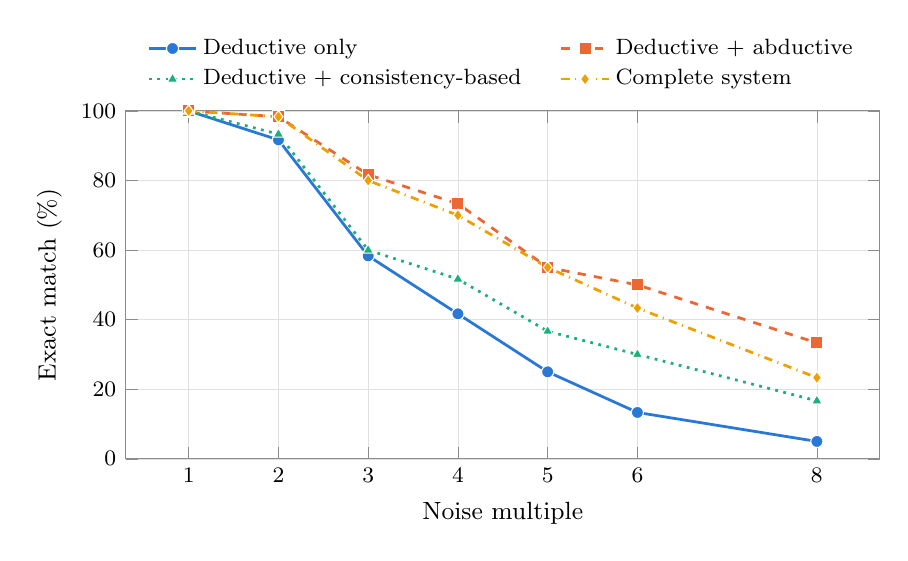
\begin{tikzpicture}
\definecolor{modedeductive}{HTML}{2a78d6}
\definecolor{modededabd}{HTML}{eb6834}
\definecolor{modededcbd}{HTML}{1baf7a}
\definecolor{modefull}{HTML}{eda100}
\begin{axis}[
  width=0.92\linewidth, height=6cm,
  xlabel={Noise multiple}, ylabel={Exact match (\%)},
  ymin=0, ymax=100,
  xtick={1,2,3,4,5,6,8},
  grid=major, major grid style={line width=0.2pt, draw=black!12},
  axis line style={draw=black!45}, tick style={draw=black!45},
  label style={font=\small}, tick label style={font=\footnotesize},
  legend style={font=\footnotesize, draw=none, fill=none, at={(0.5,1.03)}, anchor=south, legend columns=2,
    /tikz/every even column/.append style={column sep=1.2em}},
  legend cell align=left,
]
\addplot[color=modedeductive, solid, line width=1pt, mark=*, mark size=2.2pt, mark options={solid, draw=white, line width=0.4pt}] coordinates {(1,100.00) (2,91.67) (3,58.33) (4,41.67) (5,25.00) (6,13.33) (8,5.00)};
\addlegendentry{Deductive only}
\addplot[color=modededabd, dashed, line width=1pt, mark=square*, mark size=2.2pt, mark options={solid, draw=white, line width=0.4pt}] coordinates {(1,100.00) (2,98.33) (3,81.67) (4,73.33) (5,55.00) (6,50.00) (8,33.33)};
\addlegendentry{Deductive + abductive}
\addplot[color=modededcbd, dotted, line width=1pt, mark=triangle*, mark size=2.2pt, mark options={solid, draw=white, line width=0.4pt}] coordinates {(1,100.00) (2,93.33) (3,60.00) (4,51.67) (5,36.67) (6,30.00) (8,16.67)};
\addlegendentry{Deductive + consistency-based}
\addplot[color=modefull, dashdotted, line width=1pt, mark=diamond*, mark size=2.2pt, mark options={solid, draw=white, line width=0.4pt}] coordinates {(1,100.00) (2,98.33) (3,80.00) (4,70.00) (5,55.00) (6,43.33) (8,23.33)};
\addlegendentry{Complete system}
\end{axis}
\end{tikzpicture}
